\section{Results}
\label{sec:results}

This section answers the following questions:

\begin{enumerate}
\setlength{\itemsep}{-3pt}  

\item Are there applications/usage scenarios that are supported
efficiently with duty cycling.  What are the power saving achieved by
this approach?

\item What are the power savings achievable with the batching wake up approach?

\item Under what usage scenario does the customizable wakeup condition approach improve
performance (over the other approaches), and by how much?

\item What are the benefits of having customizable wakeup conditions?  
Do different applications require different wake up conditions or is
a static wake-up condition sufficient for all applications? 

\item How much additional benefit can be obtained from fully programmable wake-up conditions 
over customizable wake-up conditions based on data filtering and thresholding?

\item How dependent are the best filter/threshold combinations on the usage scenario?

\item Is the best sensor data filter choice dependant on the type of event of interest?

\item How sensitive are detection recall and energy savings to the configuration thresholds
used in the wake-up condition?

\item Are these results similar for human experiments?

\end{enumerate}

\todo[inline]{Ashvin: You need to mention earlier in the paper that you will be doing some evaluation for human traces? That was not mentioned earlier and so this comes as a surprise}

\todo[inline]{Ashvin's: Briefly restate each question at the beginning of each subsection}

\subsection{Energy Savings}

\begin{table*}[t]
    \begin{tabular}{|l|l|l|l|l|l|l|}
    \hline
	\multirow{2}{*}{~}			& \multirow{2}{*}{Approach}		& \multirow{2}{*}{\parbox{2.2cm}{Sleep Interval (seconds)}}	
																			& \multirow{2}{*}{\parbox{1.2cm}{Power (mW)}} 
																						& \multicolumn{3}{c|}{Recall} 													\\ \cline{5-7}
								&								&			&			& Walking				& Headbutt					& Transitions 				\\ \hline
	\multirow{11}{*}{Group 1}	& \multicolumn{2}{l|}{Always Awake}			& 323		& \multirow{6}{*}{98\%}	& \multirow{6}{*}{100\%}	& \multirow{6}{*}{100\%}	\\ \cline{2-4}
								& \multirow{5}{*}{Batching}		& 2			& 350		&						&							&							\\ \cline{3-4}
								& 								& 5			& 186		&						&							&							\\ \cline{3-4}
								& 								& 10		& 115		&						&							&							\\ \cline{3-4}
								& 								& 20		& 80.1		&						&							&							\\ \cline{3-4}
								& 								& 30		& 68.3		&						&							&							\\ \cline{2-7}
								& \multirow{5}{*}{Duty Cycling}	& 2			& 339		& 94\%					& 57\%						& 97\%						\\ \cline{3-7}
								& 								& 5			& 217		& 82\%					& 14\%						& 47\%						\\ \cline{3-7}
								& 								& 10		& 140		& 63\%					& 29\%						& 28\%						\\ \cline{3-7}
								& 								& 20		& 86.3		& 48\%					& 14\%						& 32\%						\\ \cline{3-7}
								& 								& 30		& 63.1		& 31\%					& 7\%						& 12\%						\\ \hline
	\multirow{11}{*}{Group 3}	& \multicolumn{2}{l|}{Always Awake}			& 323		& \multirow{6}{*}{97\%}	& \multirow{6}{*}{100\%}	& \multirow{6}{*}{100\%}	\\ \cline{2-4}
								& \multirow{5}{*}{Batching}		& 2			& 350		&						&							&							\\ \cline{3-4}
								& 								& 5			& 186		&						&							&							\\ \cline{3-4}
								& 								& 10		& 115		&						&							&							\\ \cline{3-4}
								& 								& 20		& 80.1		&						&							&							\\ \cline{3-4}
								& 								& 30		& 68.3		&						&							&							\\ \cline{2-7}
								& \multirow{5}{*}{Duty Cycling}	& 2			& 332		& 89\%					& 47\%						& 89\%						\\ \cline{3-7}
								& 								& 5			& 257		& 76\%					& 28\%						& 26\%						\\ \cline{3-7}
								& 								& 10		& 198		& 64\%					& 27\%						& 25\%						\\ \cline{3-7}
								& 								& 20		& 133		& 42\%					& 19\%						& 19\%						\\ \cline{3-7}
								& 								& 30		& 99.1		& 30\%					& 9\%						& 14\%						\\ \hline
    \end{tabular}
	\caption{Summary of achieved recall and power consumption for the Always Awake, Duty Cycling and Batching approaches}
	\label{table:summaryAA-DC-BATCHING}
\end{table*}

\begin{table}[t]
    \begin{tabular}{|l|l|l|l|}
	\hline
    ~       					& Action      & Power (mW) & Recall \\ \hline
    \multirow{3}{*}{Group 1} 	& Walking     & 48.3       & 98\%   \\ \cline{2-4}
								& Headbutts   & 60.3       & 100\%  \\ \cline{2-4}
								& Transitions & 18.6       & 100\%  \\ \hline
    \multirow{3}{*}{Group 3} 	& Walking     & 321        & 97\%   \\ \cline{2-4}
								& Headbutts   & 65.7       & 100\%  \\ \cline{2-4}
								& Transitions & 51.7       & 100\%  \\ \hline
    \end{tabular}
	\caption{Summary of achieved recall and power consumption for the Wake-up Conditions approach}
	\label{table:summaryWUC}
\end{table}

This section answers the first three questions. Table \ref{table:summaryAA-DC-BATCHING} summarizes the power and event of interest recall data for the Always Awake scenario and for various wake-up intervals for the Duty Cycling and Batching approaches. Similarly, Table \ref{table:summaryWUC} summarizes the results for the approach that uses wake-up conditions. The information in this figure represents the best wake-up conditions in terms of power consumption that achieved the same recall as the Always Awake scenario.

Duty cycling has significant drawbacks compared to other wakeup approaches. Using this approach with a sleep interval of 2 seconds actually resulted in an increase in power consumption compared to the Always Awake approach and a decrease in detection recall. This is a result of frequent transitioning between the awake and asleep states. Using sleep intervals greater than 5 seconds, we were able to obtain significant power savings. However, such long wake-up intervals caused more than a 50\% decrease in event of interest recall for infrequent events (Headbutts and Transitions) and more than 15\% decrease for step detection. We also note that in cases where the event of interest occurs rarely (group 1), the power savings of duty cycling are suboptimal because of numerous wakeups that result in no events of interest being detected. We conclude that duty cycling is not appropriate for any type of application that requires high detection recall.

Batching achieves the same event of interest recall as the Always Awake scenario, and is able to reduce power consumption for sleep intervals greater than 5 seconds. Shorter wake-up intervals can potentially cause more energy consumption than the Always Awake case because of the additional energy cost of transitioning between the sleep and awake states. Note that increasing the wake-up interval has diminishing power saving returns. A lower bound to the power consumption of the entire system is the sum of the power consumed by the main device while sleeping and the peripheral processor while being awake. Compared to the other approaches, batching has the best power savings for use cases where the event of interest occurs very frequently (i.e. walking in group 3). However, if the event of interest occurs very infrequently, batching suffers from the same problem as duty cycling. Its power consumption becomes suboptimal because of a large number of wake-ups that do not result in an event of interest being detected. Table \ref{table:summaryAA-DC-BATCHING} shows that Batching has the same power consumption regardless of activity-level (group 1 versus group 3). In this approach, events of interest are only detected after the main processor wakes up. As a result, the delay between the time when the event is occurring and the time when it is detected can be as long as the batching interval. Therefore, this approach may not be appropriate for applications that are expected to react immediately after an event of interest occurs. For example, the user of a gesture recognition application would not be satisfied if the application detects the performed gesture after a delay of more than a couple of seconds. We note that the maximum batching interval is limited by the amount of local storage available to the hardware sensor. While theoretically this approach can achieve very high energy savings (e.g. waking up every few hours), in practice realistic sleeping times are in the order of a few seconds.

When comparing the power consumption for the Duty Cycling and Batching approaches for a specific sleep interval, we need to note several things. First off, the sleep interval also includes the time spent transitioning between the awake and asleep states and vice-versa. Secondly, after a wake-up Duty Cycling keeps the phone awake for at least 4 seconds in order to collect sensor data. Batching on the other hand, only keeps the device awake for just enough time to transfer the entire batch of sensor data from the hardware sensor and to allow the application(s) to process the sensor readings. We estimated this time to be about 10\% of the sleep interval. 

% Thus, for Duty Cycling with a sleep interval of 5 seconds, the time spent awake, asleep and transitioning is 44\%, 33\% and 22\% respectively. For Batching with a sleep interval of 5 seconds, the time spent awake, asleep and transitioning is 10\%, 50\% and 40\%, respectively. Therefore, for this sleep interval, Batching results in lower power consumption. 

\begin{table*}[t]
    \begin{tabular}{|l|l|l|l|}
	\hline
    Action      					& Data Filter & Threshold \\ \hline
    Walking     					& EMA-LPF (alpha = 50\%) 						& x-axis $\geq 2 m/s^2$ 		\\ \hline
	Headbutts   					& FFT-LPF (relative energy threshold = 10\%) 	& y-axis $\leq -3.5 m/s^2$ 		\\ \hline
	\multirow{3}{*}{Transitions} 	& \multirow{3}{*}{EMA-LPF (alpha = 10\%)}		& Range Thresholds						\\ 
									&												& $2.25 m/s^2 \leq$ y-axis $\leq 3.25 m/s^2$ 	\\ 
									&												& $8.2 m/s^2 \leq$ z-axis $\leq 9.2 m/s^2$ 	\\ \hline
    \end{tabular}
	\caption{Filter-based Wake-up Conditions parameters that achieved the lowest power consumption while matching detection recall of the Always Awake approach}
	\label{table:WUCparameters}
\end{table*}

Using the customizable filter-based wake-up condition approach we were able to match the detection recall of the Always Awake approach and significantly reduce power consumption in most scenarios. In fact, this approach achieved the lowest power consumption in every scenario other than step detection in group 3. All these scenarios are similar in that the event of interest occurs infrequently (less than 15\% of the time, as seen in Figure \ref{fig:actionTimes}). Walking represents about 63\% of the courses in group 3. For this scenario, only the batching approached achieved better energy savings. Table \ref{table:WUCparameters} lists the data filter and threshold parameters that resulted in the best performance. Wake-up conditions with these parameters had the lowest power consumption while matching the detection recall of the Always Awake approach.

\subsection{Predefined Action vs Predefined Filter}

\begin{table*}[t]
    \begin{tabular}{|l|l|l|l|l|l|l|l|}
    \hline
    \multirow{2}{*}{ Wake-up condition used}
							& \multirow{2}{*}{~}	& \multicolumn{3}{c|}{Headbutts} 	& \multicolumn{3}{c|}{Transitions} 	\\ \cline{2-8}
							&						& Group 1 	& Group 2	& Group 3 	& Group 1 	& Group 2	& Group 3 	\\ \hline
    \multirow{2}{*}{Best for step detection}
							& Recall 				& 35.7\%  	& 13.0\%    & 100\%  	& 87.5\% 	& 72.6\%	& 86.0\%  	\\ \cline{2-8}
							& Power  				& 48.3 		& 177       & 321     	& 48.3 		& 177		& 321     	\\ \hline
    \multirow{2}{*}{Best custom}
							& Recall 				& 100\%   	& 100\%     & 100\%   	& 100\%   	& 100\%		& 100\%   	\\ \cline{2-8}
							& Power  				& 48.6   	& 65.1      & 65.7    	& 18.6    	& 43.3		& 51.7    	\\ \hline
    \end{tabular}
	\caption{Detection recall and power consumption for the Headbutts and Transitions actions using fixed or custom wake-up conditions}
	\label{table:predifinedActionVsPredefinedFilter}
\end{table*}

This section answers question 4. For this purpose, we assume that step detection is the one action that our hardware supports and we compare that with the benefits of custom filters for each of the other two applications. 

We start off by selecting the best wake-up condition for step detection (EMA-LPF data filter with $alpha = 50\%$ and a x-axis minimum threshold of $2\:m/s^2$, as shown in Table \ref{table:WUCparameters}). We use this wake-up condition and attempt to detect headbutts and stance transitions. The top part of Table \ref{table:predifinedActionVsPredefinedFilter} shows the results in terms or detection recall and power consumption. In the bottom half of the table we present the results for the same metrics when we used the best wake-up condition for those specific actions (see Table \ref{table:WUCparameters}). 

We note that in every single case, using a custom filter increased detection recall and in most cases reduced power consumption. For the headbutt action, recall more than doubled for groups 1 and 2. For group 3, the wake-up condition used for step detection resulted in all headbutts being detected. However, this required almost 400\% additional power usage compared to the best custom wake-up condition for headbutts. For transitions, using a custom filter increased recall to 100\% for every group and reduced power consumption by at least a factor of 2.5. In terms of power consumption the best results are visible in group 3, the group with the highest amount of walking. In group 3, the energy consumption was reduced by approximately 84\%.

We can conclude that using a fixed wake-up condition (or predefined hardware supported action detection) may work well for a small set of application, but is inefficient for most other applications. As such, developers should be able to configure the wake-up conditions based on the needs of their applications. 

\subsection{Customizable filter-based wake-up condition vs Oracle}

\begin{table*}[t]
    \begin{tabular}{|l|l|c|c|c|c|c|}
	\hline
    ~       					& Action      & Recall 	& \parbox{3.0cm}{Power Usage Oracle Wake-up Condition} 
																	& \parbox{3.0cm}{Power Usage Custom Wake-up Condition} 
																				& \parbox{2.5cm}{Additional savings by Oracle} 
																							& \parbox{2.5cm}{Savings as \% of Always Awake}\\ \hline
    \multirow{3}{*}{Group 1} 	& Walking     & 98\%   	& 41.5      & 48.3		& 6.8		& 2.1\% \\ \cline{2-7}
								& Headbutts   & 100\%  	& 59.6      & 60.3		& 0.7		& 0.2\% \\ \cline{2-7}
								& Transitions & 100\%  	& 16.4      & 18.6		& 2.2		& 0.7\% \\ \hline
	\multirow{3}{*}{Group 2} 	& Walking     & 99\%  	& 153       & 188		& 35		& 10.9\% \\ \cline{2-7}
								& Headbutts   & 100\%  	& 62.6      & 65.1		& 2.5		& 0.8\% \\ \cline{2-7}
								& Transitions & 100\%  	& 29.5      & 43.3		& 13.8		& 4.3\% \\ \hline
    \multirow{3}{*}{Group 3} 	& Walking     & 97\% 	& 266       & 321		& 55		& 17.0\% \\ \cline{2-7}
								& Headbutts   & 100\%  	& 62.9      & 65.7		& 2.8		& 0.9\% \\ \cline{2-7}
								& Transitions & 100\%  	& 34.9      & 51.7		& 16.8		& 5.2\% \\ \hline
    \end{tabular}
	\caption{Comparison of power savings using a perfect Wake-up Condition (Oracle) versus the best custom filter-based wake-up condition}
	\label{table:WUCoracle}
\end{table*}

This section answers question 5. We wanted to examine how much additional benefit can be obtained from fully programmable wake-up conditions over the customizable wake-up conditions based on data filtering and thresholding. A fully-programmable wake-up condition has the potential to be "perfect". That is, it will only wake up the device if and only if an event of interest will be detected by the application (i.e. 100\% wake-up precision). Such a wake-up condition will achieve the lowest possible power consumption while matching the detection recall of the Always Awake approach. We will refer to this wake-up condition as the Oracle. Such an wake-up condition could be implemented by moving most of the functionality of the application to the low-power processor. However, this approach has significant limitations, as described in Section~\ref{subsec:computationOffloading}.

We used the list of events detected by the Always Awake simulations to determine the awake time, asleep time and number of wake-ups for the Oracle wake-up condition. These values were then used to estimate power consumption. Table \ref{table:WUCoracle} compares the power compunction of the Oracle with the power consumption for the best custom filter-based wake-up condition presented earlier. The difference between these values represents how much additional power savings can potentially be achieve by allowing developers full-programmability of the wake-up conditions. Table \ref{table:WUCoracle} also presents this difference as a percentage of the power consumption of the Always Awake approach. For most usage scenarios, having an Oracle wake-up condition results in less that 5.5\% additional power savings. For high-frequency events (walking in groups 2 and 3), the Oracle has significantly more power savings, 10.9\% and 17.0\%, respectively.

\subsection{Usage Dependence}

\begin{figure}[h]
	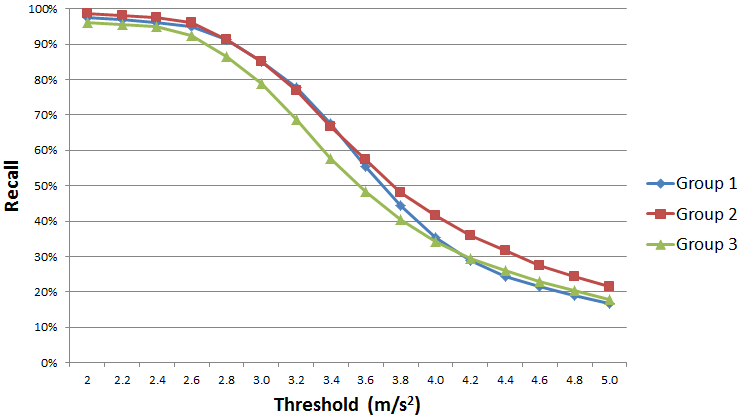
\includegraphics[width=8.5cm]{wuc_steps_recall_by_group_and_th.png}
	\caption{}
    \label{fig:wucStepsRecallByGroupAndThreshold}
\end{figure}

This section answers question 6. Figure \ref{fig:wucStepsRecallByGroupAndThreshold} shows the step recall based on the wake-up condition threshold value for each of the groups. We note that for different usage scenarios (i.e. each of the groups), the recall does not change by more than 10\% for any given threshold value. Similar results were found for all the events of interest. 

We conclude that the best filter and threshold combinations are not dependent on the usage scenario.

\subsection{Sensor Data Filter Choice}

\begin{table*}[t]
    \begin{tabular}{|l|l|c|c|c|c|c|}
	\hline
    \multirow{2}{*}{Sensor Data Filter}    	& \multicolumn{3}{c|}{Power Consumption (mW)} \\ \cline{2-4}
							& Walking	& Headbutts	& Transitions 	\\ \hline
    Null     				& 191		& 186		& 67.8 			\\ \hline
	EMA-LPF   				& 188		& 228		& 43.3 			\\ \hline
	FFT-LPF 				& 217		& 65.1 		& 88.7 			\\ \hline
	
    \end{tabular}
	\caption{Summary of best achieved power consumption for each of the sensor data filters for Group 2}
	\label{table:WUCfilters}
\end{table*}

This section answers question 7. Table \ref{table:WUCfilters} lists the best achieved power consumption by the Custom filter-based Wake-Up Condition approach using each of the sensor data filters, while matching the detection recall of the Always Awake approach. We observe that the best and worst sensor data filter changes depending on the event of interest. The Null filter had the second best power consumption for all of the applications. The EMA-LPF has the lowest power consumption for the Walking and Transitions applications, while the FFT-LPF had the lowest power consumption for the Headbutts application. 

We observe that different data filters are optimal for different applications. Even in cases where the same filter type is optimal, the configuration parameters for the filter and the wake-up thresholds may be different. Additionally, applications might only be interested in the acceleration values on specific axes, preventing the same filter from being shared with other applications.

\subsection{Wake-up Threshold Sensitivity}

\begin{figure}[h]
	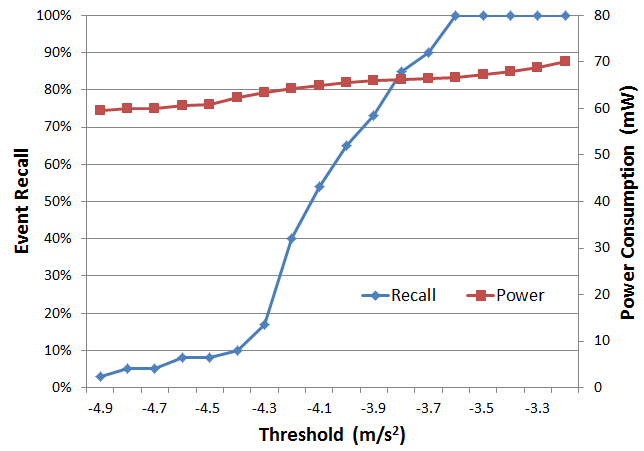
\includegraphics[width=8.5cm]{wuc_hb_fft_group3.png}
	\caption{}
    \label{fig:wucHeadbuttFFTRecallPowerGroup3}
\end{figure}

This section answers question 8. Figure \ref{fig:wucHeadbuttFFTRecallPowerGroup3} shows the detection recall and power consumption for the Headbutt application using the best wake-up condition. Similar graphs were generated for the other applications, but were omitted due to lack of space. We note that the choice of threshold is important, as choosing a threshold that is too strict will cause a significant drop-off in the achieved recall. However, choosing a threshold that is too lenient will result in additional power consumption without any extra benefit to recall because of unnecessary wake-ups. 

\subsection{Macrobenchmarks}

\begin{table*}[t]
    \begin{tabular}{|l|c|c|c|c|c|c|}
    \hline
	\multirow{2}{*}{Approach}		& \multirow{2}{*}{\parbox{2.2cm}{Sleep Interval (seconds)}}
												& \multicolumn{3}{c|}{\parbox{1.2cm}{Power (mW)}}
																								& \multirow{2}{*}{\parbox{1.5cm}{Average Recall}} \\ \cline{3-5}
									&			& Trace 1		& Trace 2		& Trace 3 		& 							\\ 
									&			& 35\% - 45\% walking	& 20\% - 30\% walking		& 20\% - 30\% walking		& \\ \hline
	Always Awake					& 			& \multicolumn{3}{c|}{323} 						& 100\% \\ \hline
	\multirow{5}{*}{Duty Cycling}	& 2			& 329			& 330			& 330			& 97\%	\\ \cline{2-6}
									& 5			& 272			& 260			& 261			& 92\%	\\ \cline{2-6}
									& 10		& 220			& 195			& 198			& 82\%	\\ \cline{2-6}
									& 20		& 172			& 131			& 134			& 66\%	\\ \cline{2-6}
									& 30		& 148			& 104			& 106			& 57\%	\\ \hline
	\multirow{5}{*}{Batching}		& 2			& \multicolumn{3}{c|}{350} 						& 100\% \\ \cline{2-6}
									& 5			& \multicolumn{3}{c|}{186} 						& 100\% \\ \cline{2-6}
	 								& 10		& \multicolumn{3}{c|}{115} 						& 100\% \\ \cline{2-6}
	 								& 20		& \multicolumn{3}{c|}{80.1} 					& 100\% \\ \cline{2-6}
	 								& 30		& \multicolumn{3}{c|}{68.3} 					& 100\% \\ \hline
	Wake-up Condition				&			& 136			& 77.9			& 72.6			& 100\% \\ \hline
    \end{tabular}
	\caption{Summary of achieved recall and power consumption for each wake-up approach for macrobenchmarks}
	\label{table:macrobenchmarks}
\end{table*}

This section answers question 9. We collected three accelerometer traces of three different individuals performing routine daily activities. The first trace is 2 hours and 10 minutes long captured during an individual's morning commute. The second trace is 1 hour and 2 minutes long and captured by a person working in a retail store. The third trace is 3 hours and 17 minutes long, captured by a person working in an office environment. Roughly 20\% to 45\% of each trace is spent walking. This usage scenario is similar with walking in groups 2 and 3 for the microbenchmarks. 

Table \ref{table:macrobenchmarks} shows a summary of the results obtained by running the simulator using these traces. Since ground truth information is not available, detection recall is determined by comparing the steps detected by each wake-up approach with those detected by the Always Awake approach.

The Always Awake approach is used as a baseline. The estimated power consumption for this approach is 323 mW.

The results for Duty Cycling are almost identical to the results of the microbenchmarks. Using a sleep interval of 2 seconds results in a detection recall above 95\%, but it uses more power than the Always Awake approach because of frequent device wake-ups. Increasing the sleep interval results in some power savings, but at a significant cost to detection recall.

The results for Batching and Custom Filter-Based Wake-up Conditions are similar to the microbenchmarks results for step detection in group 3, where the event of interest was very frequent. Both Batching and the best Wake-up Condition match the performance of the Always Awake approach (detecting the same steps) and both have significant power savings. The lowest power consumption was achieved by batching with a sleep interval of 30 seconds. The best custom filter-based wake-up conditions also achieved more than 55\% power savings in each of the traces. Batching has the best performance because in only requires about 10\% awake time, compared to wake-up conditions for which the awake time is proportional to the frequency of events on interest. However, batching introduces a delay between the time when the event occurs and the time when it is detected by the application. While this drawback is tolerable for the Pedometer application used in our experiments, it may be unacceptable for other types of applications. 

We conclude that these results are similar to their microbenckmark counterparts.


